\chapter{Introduction}
\label{introduction}

As the efficiency and accuracy of rapid genome sequencing skyrockets, the potential for personalized therapies has made its way from science fiction to scientific reality. Using genetics to understand, diagnose, and eventually to predict illness is not a new idea; in recent years, however, technological ability and scientific understanding have advanced to such a point that researchers may predict risk for several diseases with reasonable confidence. Increasingly, variants in the human genome are being identified as being robustly linked to risk for complex illnesses such as heart disease [\small{cite 9p21}], obesity [\small{cite fto}], and schizophrenia [\small{cite something}]. However, much work remains to be done in order to create tools which may accurately predict individual disease risk from known and unknown genetic risk factors. In this thesis, we propose a novel extension to a well known methodology in order to better characterize disease risk from comorbid conditions using only summary statistics. 

In brief, we present preliminary evidence for the use of \ac{PRS}s in predicting \ac{CAD}. We use recently published summary statistics from a \ac{GWAS} conducted by the \ac{CARDIOGRAMC4D} consortium alongside evidence gathered by the \ac{GLC} and the \ac{GIANT} consortium for lipids and \ac{BMI} \textit{per say}. We use this data alongside previously identified variants to construct first a simplistic \ac{PRS} using only genome wide statistically signficant ($P_{Bonferonni} < 0.05$ or $q_{FDR}$ < 0.05) variants, then expand our search to variants which may not be as robustly linked to phenotype. [Cite storey, BH, and dudbridge]. We use an empirical maximation approach and several strategies of mathematical optimization in order to construct an \ac{oPRS}, then devise a novel technique for integrating information from co-morbid \ac{oPRS} diseases in order to better predict \ac{CAD} in four cohorts comprising approximately $n=12,000$ individuals

\section{Genetics of Coronary Artery Disease}

\ac{CAD} occurs when the major blood vessels supplying the heart become diseased or damaged, often leading to severe complications such as \ac{MI} and death. [cite review articles] \ac{CAD} is known to be a complex genetic disease with heritability estimated by twin studies between 40 and 60\%. [mcPherson 2016, twin studies paper] Several important variants have been indentified which have been shown to robustly increase risk to \ac{CAD} by altering lipid transporting pathways [cite LDLR], structural collegan bodies [TRIB 1??], and others factors. 


\begin{figure}[h]
\caption{Progression of the formation of plaque causing \ac{CAD}. Adapted from Gretch 2003.}
\centering
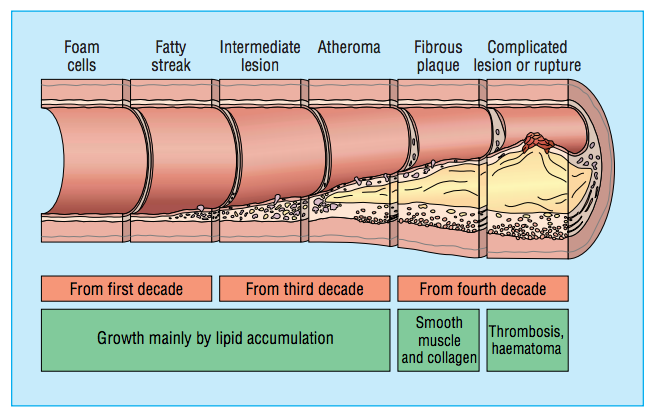
\includegraphics[width=0.8\textwidth]{Figures/cad.png}
\end{figure}

With heart disease and stroke the leading cause of perscription drug use in Canada as well as one of the leading causes of death and hospitalization [cite herat and stroke], the need to better understand, diagnose, and prevent this deadly disease is apparent.  In order to better understand the need for improved statistical methodologies, it is important to understand the large body of previous attempts to characterize the genetic determinants of \ac{CAD}

Despite some promising beginings, initial attempts to understand and explain \ac{CAD} through genetics were largely unsuccessful.[CITE] The first variant to be succesfully and robustly linked to risk for \ac{CAD} was the 9p21.3 locus. Discovered by a team of researchers at the Univeristy of Ottawa Heart institute, the allele consists of a 58 \ac{kb} region on chromosome 9 which was shown to be associated with \ac{CAD} in a population of 23,000 caucasion individuals. (\cite{McPherson2016})

\begin{figure}[h]
\caption{Fine mapping of the genomic interval on chromosome 9 associated with Coronary Heart Disease. Adapted from Mcpherson et al 2006}
\centering
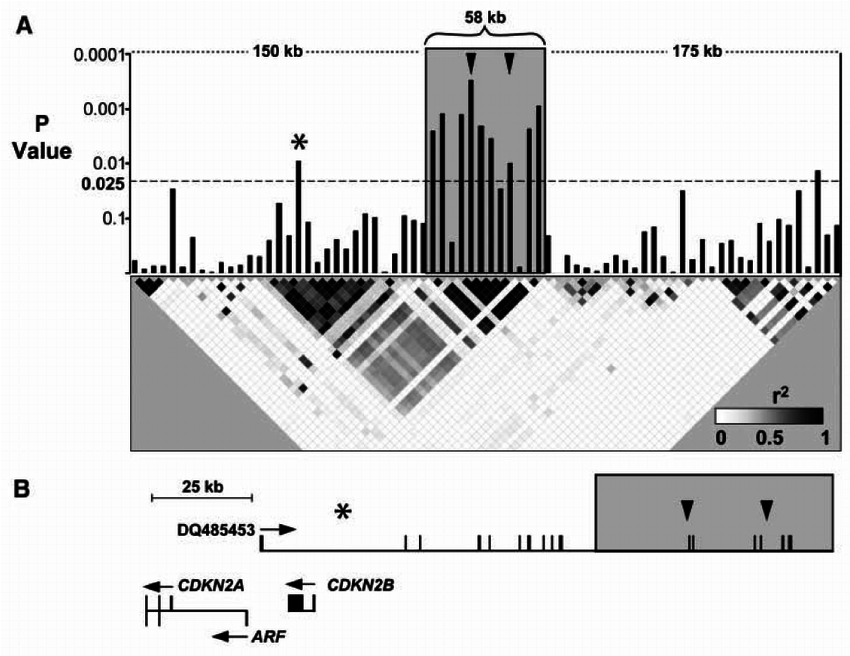
\includegraphics[width=0.8\textwidth]{Figures/9p21.png}
\end{figure}

This initial success began the era of the \ac{GWAS}, explained in more detail in section \ref{gwas}.  Researchers across the globe began frantically searching for more loci with the hope of understanding and predicting complex disease; in that goal, the \ac{GWAS} has failed. (\cite{Visscher2012}) A number of important genetic markers for \ac{CAD} have been discovered, but often in small familial cases or with very low effect sizes. [Cite] As the dust settles and the low hanging fruit have been picked, common variants have been shown to explain approximately 28\% of the heritablity of \ac{CAD} [cite majid], yet a large portion remains to be accounted for. This has become known as the problem of ``missing heritabillity'' of complex disease; common genetic variants explain a relatively small portion of the total estimated heritability of a disease, therefore researchers must resort to ever more obscure and complex methods to attempt to explain the complex interactions between genetic elements in the human genome. [cite review paper] From pathway analysis to partitioned heritability to all kinds of arcane statistical procedures, researchers from across the globe have tried their hardest to shrink this gap between our knowledge and accurate prediction and understanding of complex disease. To this end, we develop our own methodology incorporating multiple sources of information for the more accurate prediction of clinical end points. 

\section{Genome Wide Association Studies} \label{gwas}

In order to properly introduce the model, however, the basic underpinnings must be explored and explained. Genome wide association studies seek to indetify associations between individual genotypes and disease phenotypes in a hypothesis free manner. In this section, the statistical model required to understand \ac{GWAS} is presented and explored.

\subsection{Primer on Genetics}

\ac{DNA} is a double helical molecule which encodes the genetic blueprints for the construction of proteins and other materials that make up every known living organism. \ac{DNA} is composed of three parts: a negatively charged phosphate group, a five carbon sugar \textit{deoxyribose}, and (usually) one of four nitrogen bases. It is these bases, \ac{A}, \ac{C}, \ac{T}, and \ac{G} and their combinations which are under investigation in a \ac{GWAS}. The specific combinations of these four bases in a \ac{locus} determine the product produced by the \ac{DNA}, and even a small change in this order can have large ramifications on the overall health, survival, and proper function of the organism. 

\subsection{Sequencing}

DNA sequencing is the process of ascertaining a particular individual's genotype by means of chemical identification of the bases present at predefined sites. [cite] These sites, whether they be a change in a single base called a \ac{SNP}, a variation in the number of tandem repeats of a small sequence named a \ac{CNV} or an \ac{InDel} of a sequence, may alter amino acid sequence, affect regulatory regions, or impact regulatory \ac{RNA} sequences.

\begin{definition}[Allele]
A specific form or subtype of a genetic locus. This could be one or more individual variations or a combination therof. 
\end{definition}

\begin{rem}
Allele frequency is the frequency at which a particular allele occurs in the population. I.e. for locus $A$ having $n$ different alleles, the true population allele frequency of allele $freq A_m \equiv \frac{A_m}{ \sum^n_{i=1} A_i}$, which is estimated in a sample population with a biased ratio estimator $freq \hat{A}_m \equiv \frac{\hat{A}_m}{ \sum^n_{i=1} \hat{A}_i}$  
\end{rem}

\subsection{Statistical Definition}

Consider a simple case control population where 1 defines case and 0 defines control. Define $\underline{\mathbf{Y}}$ as an $n$-vector where $n$ denotes the number of individuals in a population and $\underline{\mathbf{Y}}_i$ gives the individual's diesease staet. Additionally define $G$ as an $m \times n$ matrix where $m$ is the number of informative genotypic sites available with $\mathbf{G}_{ij}$ being the ``state'' (allele number) present at site $j, 1 \leq i \leq m, i \in \mathbb{Z}^+$ in individual $i, 1 \leq i \leq n, i \in \mathbb{Z}^+$.

$$ \begin{aligned} &\mathbf{\underline{Y}} &= \begin{bmatrix} Y_1 \\ \vdots \\ Y_n \end{bmatrix} \, \, \, \, \, \, \, \,\, \, \, \,\, \, \, \, \, \, \, \, \, \, \, \,\, \, \, \,\, \, \, \, &  \mathbf{G} &= \begin{bmatrix} G_{1,1} & \dots & G_{1, n} \\ \vdots & \ddots & \vdots \\ G_{m, 1} & \dots & G_{m, n} \end{bmatrix} \end{aligned} $$

In an additive genetic model, we define the phenotype $\underline{\mathbf{Y}}$ as a linear combination of $\mathbf{G}$ weighted by a vector of $\underline{\mathbf{\beta}}$ coefficicent vectors estimated by regression analysis and $\underline{\mathbf{\epsilon}}$ vector of errors. Express $\underline{\mathbf{Y}}$ such that

$$ \underline{\mathbf{Y}} = \underline{\mathbf{\beta}}' \mathbf{G} + \underline{\mathbf{\epsilon}} = \left( \sum^m_{i=1} \beta_i \mathbf{G}_{i, n} + \epsilon_n \right)' $$

$\underline{\mathbf{\beta}}$ and $\underline{\mathbf{\epsilon}}$ are approximated optimally by $\underline{\hat{\beta}}$ and $\underline{\hat{E}}$ in practice.

The purpose of a \ac{GWAS} is not only to estimate these genetic effects $\underline{\mathbf{\beta}}$ by $\underline{\hat{\beta}}$ but also to estimate their significance of association with phenotype vector $\underline{\mathbf{Y}}$ through a $\chi^2$ test and corresponding test statistic $m$-vector $\hat{\chi}^2$. The degrees of freedom of this test statistic will vary between methods and models, and so will be left as futher reading. 

By approximating $\underline{\chi^2}$ with $\hat{\underline{\chi^2}}$ and computing the corresponding $P$ values, reserchers are able to identify and quantify the effects of variants significantly ($P < 0.05$) associated with the phenotype. These results can be summarized in a Manhattan plot, named after the city of Manhattan with it's high rise buildings towering over the scenery. The $x$ axis of this plot is the genomic location (usually coloured by chromosome number) while the $y$ axis is the $\log_{10}$ of the $P$ value of association derived from $\hat{\underline{\chi^2}}$. 


\begin{figure}[H]
\caption{Example of a Manhattan plot from a \ac{GWAS} for \ac{CAD} performed by Shunkert et al. 2011}
\centering
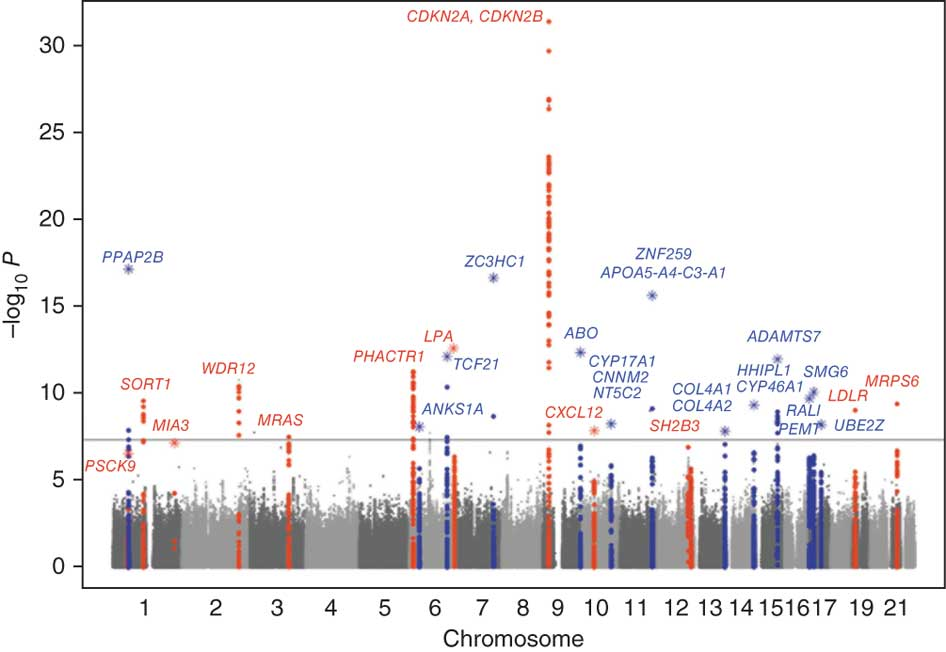
\includegraphics[width=0.5\textwidth]{Figures/man_ex.jpg}
\end{figure}

\subsection{Multiple Comparisson Problem}

In such a set up, where $m$ may be in the millions and the threshold of significance is set to $P = \alpha = 0.05$, we encounter a canonical issue in statistical inference. Recall that $P$ is the probability of observing a $\chi^2$ statistic as large or larger than a specific $\chi^2_m$ assuming $H_0$ of no association is correct and $\alpha$ is the threshold at which a significant effect is declared. 

For the sake of description, we define $M$ as the number of \textit{independant} variants (that is, the effective number of variants which are not in \ac{LD})

\section{Polygenic Prediction of Complex Disease}

Refering to the defintions proposed in the previous section and recalling that 

\section{Polygenic Sliding Window Optimization}
\section{Summary}